\documentclass[11pt]{article}

\usepackage[margin=1in]{geometry}
\usepackage{graphicx}
\usepackage{booktabs}
\usepackage{amsmath}
\usepackage{siunitx}
\usepackage{hyperref}
\usepackage{caption}
\usepackage{float}

\graphicspath{{figures/}}
\hypersetup{colorlinks=true,linkcolor=blue,citecolor=blue,urlcolor=blue}
\setlength{\emergencystretch}{2em}

\title{Validation and Acceleration of an ecape-parcel-Compatible Solver for HRRR-Scale Entraining-CAPE Diagnostics}
\author{ECAPE-RS Project}
\date{25 April 2026}

\begin{document}
\maketitle

\begin{abstract}
Full entraining parcel-path ECAPE calculations are useful for diagnosing diluted convective updraft buoyancy, but public implementations have generally been practical at individual-sounding scale rather than HRRR-grid scale. We developed a Rust implementation intended to reproduce the public, Peters-checked \texttt{ecape-parcel} Python parcel-path calculation while reducing the cost of the calculation enough for profile batches, full-grid maps, and archive-scale severe-weather diagnostics.

The implementation was evaluated with a direct parity harness against \texttt{ecape-parcel} 1.2.2. The harness compares raw \SI{20}{m} parcel paths, density temperature, buoyancy, integrated positive buoyancy, CIN, LFC, EL, and runtime for surface-based, mixed-layer, and most-unstable parcel sources under entraining/non-entraining and pseudoadiabatic/irreversible ascent modes. The harness also found and fixed mixed-layer-origin and humidity-construction incompatibilities.

After those fixes, a synthetic no-entrainment limit test passed for all SB/ML/MU pseudo/irreversible combinations with $|\Delta E|<10^{-9}\ \mathrm{J\,kg^{-1}}$. A 6 May 2024 HRRR warm-sector profile agreed within \SI{0.041}{J\,kg^{-1}} across all 12 parcel-source/ascent-mode configurations, with maximum parcel-density-temperature differences below $4\times10^{-5}\ \mathrm{K}$. A first event-sample parity sweep then ran 252 profile cases and 3,024 configurations, including the synthetic fixture, the single HRRR 2024-05-06 test profile, 50 tornado target profiles, and 200 displaced controls. All configurations passed the first-stage criteria. A bounded v2 sweep added 100 random HRRR profiles, a 10-profile stress suite, and four storm-motion modes, producing 5,368 comparable configurations with zero first-stage parity failures and eight separately recorded \texttt{ecape-parcel} reference exceptions.

The measured Python parcel-path package calls took 2.8--6.1 s per configuration on the HRRR profile, while the Rust solver took about 0.45--0.65 ms, implying speedups of roughly $5{,}600$--$13{,}000\times$ for this benchmark. Four 272,955-cell full-grid pilot cases each processed in 17.6--18.4 s. These results support the main methods claim: \texttt{ecape-parcel} provides a public sounding-scale parcel-path reference implementation, and a compatible Rust implementation makes the same class of calculation practical for HRRR-grid diagnostics and archive-scale ECAPE research.
\end{abstract}

\section{Introduction}

Entraining convective available potential energy (ECAPE) is valuable because real convective updrafts entrain environmental air. Traditional CAPE is an undiluted parcel-theory diagnostic; it does not directly represent dilution, condensate loading, or the way storm-relative flow can affect an updraft. Peters et al. \cite{peters2023ecape} developed an analytic ECAPE formulation in which entrainment is linked to the environmental sounding, storm-relative flow, updraft geometry, and mass continuity.

The public Python package \texttt{ecape-parcel} made a related full parcel-path calculation accessible to sounding users. Its project description states that it computes ECAPE values and parcel paths, supports entraining and non-entraining pseudoadiabatic and irreversible ascent modes, and was checked against Peters's \texttt{ECAPE\_FUNCTIONS} script \cite{ecapeparcel}. The documentation also emphasizes that density temperature should be plotted, not just parcel temperature, because Peters's formulation accounts for condensate effects on parcel density \cite{ecapeparcel}. SounderPy then exposed this toolkit in an advanced sounding workflow, allowing users to plot surface-based, mixed-layer, and most-unstable ECAPE/CAPE parcels \cite{sounderpyparcels}.

That lineage motivates the central methods claim:

\begin{quote}
Peters provides the theory and analytic approximation. \texttt{ecape-parcel} provides the public, Peters-checked parcel-path implementation. \texttt{ecape-rs} provides a compatible high-throughput Rust implementation for HRRR-grid and archive-scale science.
\end{quote}

The first question is therefore methodological:

\begin{quote}
Can the public, Peters-checked \texttt{ecape-parcel}-style entraining parcel calculation be reproduced at HRRR-grid speed?
\end{quote}

Only after that question is answered should the second scientific question take over:

\begin{quote}
Once full parcel-path ECAPE is cheap, where does it differ from Peters analytic ECAPE, and do those differences matter meteorologically?
\end{quote}

\section{Definitions}

This manuscript separates three ECAPE families.

\begin{description}
  \item[Peters analytic ECAPE, $E_{\mathrm{analytic}}$.] The scalar analytic ECAPE diagnostic derived from the environmental profile and storm-relative-flow assumptions.
  \item[ecape-parcel-style parcel-path energy, $E_{\mathrm{parcel}}$.] The integrated positive buoyancy along a full entraining parcel path, using the \texttt{ecape-parcel} family of assumptions.
  \item[Rust parcel-path energy, $E_{\mathrm{rust}}$.] The Rust implementation of the same class of parcel-path calculation.
\end{description}

The main path-energy diagnostic is

\begin{equation}
E_{\mathrm{parcel}} =
\int_{z_{\mathrm{LFC}}}^{z_{\mathrm{EL}}} \max(B_e(z),0)\,dz,
\end{equation}

where

\begin{equation}
B_e(z)=g\frac{T_{\rho,p,e}(z)-T_{\rho,env}(z)}{T_{\rho,env}(z)}.
\end{equation}

Here $T_{\rho,p,e}$ is the density temperature of the entraining parcel and $T_{\rho,env}$ is the density temperature of the environment. This notation avoids the weak internal label ``explicit +B'' and keeps the final diagnostic tied to the ecape-parcel/Peters density-temperature framing.

The analytic-versus-full-path difference is defined as

\begin{equation}
\Delta E = E_{\mathrm{parcel}} - E_{\mathrm{analytic}}.
\end{equation}

\section{Methods}

\subsection{ecape-parcel as the Reference Parcel-Path Implementation}

The installed Python reference package in this environment was \texttt{ecape-parcel} 1.2.2. It was called directly with

\begin{verbatim}
from ecape_parcel.calc import calc_ecape_parcel,
    density_temperature, custom_cape_cin_lfc_el
\end{verbatim}

The parity harness passes the same pressure, height, temperature, dewpoint, and wind arrays to Python and Rust. It then writes a normalized schema containing environmental profile metadata, parcel pressure/height/temperature/water-vapor/total-water arrays, parcel density temperature, environmental density temperature interpolated onto the parcel path, buoyancy, $E_{\mathrm{parcel}}$, CIN, LFC, EL, parcel source, ascent mode, storm-motion mode, and runtime.

\subsection{Rust Compatibility Harness}

The Rust side uses the vendored \texttt{ecape-rs} runner and returns the same normalized fields. Both paths are compared on a common \SI{20}{m} height grid when necessary. For each profile/configuration, the harness computes maximum and mean parcel-temperature error, maximum and mean density-temperature error, maximum and mean buoyancy error, $E_{\mathrm{parcel}}$ difference, CIN difference, LFC/EL differences, runtime, and zero-versus-nonzero mismatch flags.

The first harness runs immediately found important compatibility issues. The Rust mixed-layer parcel source used a pressure-weighted/mixing-ratio construction, while \texttt{ecape-parcel} averages potential temperature and specific humidity over the included mixed-layer levels. A second pass found that Rust was rebuilding mixed-layer dewpoints from specific humidity before averaging, while \texttt{ecape-parcel} averages the MetPy specific humidity computed directly from the original dewpoints. The Rust mixed-layer origin and humidity path were changed to match \texttt{ecape-parcel}. This is exactly why the parity harness needs to be a first-class part of the project rather than an afterthought.

\subsection{Reproducibility State}

The tables and figures in this manuscript were generated from JSON/CSV parity outputs under \path{ecape_method_validation_20260425}. The first target/control sweep is stored in \path{parity_sweep_v1_target_control}; the bounded random/stress/storm-motion v2 outputs are stored in \path{parity_sweep_v2_random100_matrix}. At the time of this manuscript build, the standalone \texttt{ecape-rs} repository was based on commit \texttt{50b9366} and the \texttt{rustwx} repository was based on commit \texttt{72766fc}, with the parity harness using \texttt{ecape-parcel} 1.2.2. The random v2 sweep used seed \texttt{20260426}; the formal large random/stress sweep should preserve its input-profile manifest, parity-summary CSV files, reference-exception table, and worst-case diagnostic plots with the manuscript artifacts.

\subsection{First-Stage Acceptance Criteria}

For this initial method check, a configuration is treated as passing first-stage parity when $|\Delta E_{\mathrm{parcel}}| < \SI{2}{J\,kg^{-1}}$, maximum $|\Delta T_\rho| < \SI{0.01}{K}$, and there is no zero/nonzero LFC/EL or path-energy mismatch. These tolerances are meteorologically small relative to typical ECAPE magnitudes in the tested cases and to the earlier target/control differences of hundreds of \si{J\,kg^{-1}}; the density-temperature threshold corresponds to a very small buoyancy perturbation along the parcel path. These are not final universal-verification criteria; they are a practical screen for identifying implementation mismatches before the larger archive parity sweep.

An internal no-entrainment-limit test was also added to the Rust test suite. With entrainment disabled, the parcel-path positive-buoyancy integral must match the Rust continuous path CAPE calculation on the same \SI{20}{m} path for each parcel source and ascent mode. This is separate from Python/Rust parity; it checks the simplest physical limit inside the Rust solver.

\begin{table}[H]
\centering
\caption{Internal no-entrainment-limit tests on the synthetic parity fixture.}
\label{tab:noentrainment}
\begin{tabular}{llrl}
\toprule
Test & Parcel/mode & Max $|\Delta E|$ & Result \\
 & & (J\,kg$^{-1}$) & \\
\midrule
Continuous CAPE path limit & SB non-entraining pseudo & $<10^{-9}$ & Pass \\
Continuous CAPE path limit & SB non-entraining irrev. & $<10^{-9}$ & Pass \\
Continuous CAPE path limit & ML non-entraining pseudo & $<10^{-9}$ & Pass \\
Continuous CAPE path limit & ML non-entraining irrev. & $<10^{-9}$ & Pass \\
Continuous CAPE path limit & MU non-entraining pseudo & $<10^{-9}$ & Pass \\
Continuous CAPE path limit & MU non-entraining irrev. & $<10^{-9}$ & Pass \\
\bottomrule
\end{tabular}
\end{table}

\subsection{Compatibility Fixes Found by the Harness}

The parity harness was useful because it exposed implementation mismatches rather than merely confirming expected behavior. Table~\ref{tab:fixes} lists the main compatibility fixes that moved the Rust implementation toward \texttt{ecape-parcel} behavior.

\begin{table}[H]
\centering
\small
\caption{Compatibility issues found and fixed by direct \texttt{ecape-parcel}/Rust parity testing.}
\label{tab:fixes}
\begin{tabular}{>{\raggedright\arraybackslash}p{0.20\textwidth}>{\raggedright\arraybackslash}p{0.23\textwidth}>{\raggedright\arraybackslash}p{0.28\textwidth}>{\raggedright\arraybackslash}p{0.18\textwidth}}
\toprule
Issue found & Symptom & Fix & Effect \\
\midrule
Mixed-layer source & Mixed-layer parcel offset & Match \texttt{ecape-parcel}/MetPy potential-temperature and humidity averaging & ML parity improved \\
Humidity path & Dewpoint roundtrip changed mixed-layer humidity & Preserve direct specific-humidity construction where available & Synthetic and ML offsets reduced \\
Most-unstable selection & MU origin outliers & Match MetPy-style layer selection and equivalent-potential-temperature ranking & MU outliers removed \\
Zero-CAPE entraining path & Empty-path and LFC/EL zero/nonzero mismatches & Return the reference empty entraining path when undiluted CAPE is nonpositive & Mismatch flags removed \\
Storm motion / VSR & Small entrainment-rate offsets in entraining modes & Match MetPy-style Bunkers layer averaging for reference storm motion & Entraining-mode residuals reduced \\
\bottomrule
\end{tabular}
\end{table}

\subsection{HRRR Data and Severe-Weather Pilot}

The HRRR demonstration used archived surface and pressure-level model fields. NOAA describes HRRR as a real-time 3-km, hourly updated, cloud-resolving, convection-allowing model with 3-km radar assimilation \cite{hrrrweb}. A profile probe extracts a surface-augmented HRRR column, computes parcel diagnostics, and can now optionally write the full input column so the Python/Rust parity harness can be run on the same model profile.

The severe-weather pilot used 50 tornado-associated HRRR target profiles and four same-hour displaced controls per target. The profiles were drawn from the existing top-50 tornado-associated HRRR probe archive, spanning HRRR initialization dates from 23 February 2016 through 2 April 2025, forecast hours 0--6, and 00, 18, and 21 UTC cycles. The four controls were displaced from each target by fixed offsets: north $(+0.9^\circ, 0.0^\circ)$, east $(0.0^\circ, +0.9^\circ)$, northwest $(+0.8^\circ, -0.8^\circ)$, and southeast $(-0.8^\circ, +0.8^\circ)$ in latitude/longitude. Each probe used the same HRRR cycle, forecast hour, and surface/pressure-field merge as its target. This is a conservative local-control design, not a benign/null verification dataset. It tests whether tornado report points differ from nearby same-setup environments.

\section{Compatibility Results}

Table~\ref{tab:parity} summarizes the direct \texttt{ecape-parcel} versus Rust harness results after the compatibility fixes. The HRRR 6 May 2024 profile agreed within \SI{0.041}{J\,kg^{-1}} across all 12 parcel-source/ascent-mode combinations, with maximum density-temperature differences of only $4\times10^{-5}\ \mathrm{K}$.

The synthetic parity-column fixture now agrees within \SI{0.41}{J\,kg^{-1}} across all 12 configurations, with maximum density-temperature differences below $4\times10^{-4}\ \mathrm{K}$. The \texttt{ecape-parcel} documentation reports that its parcel-path comparison to Peters's reference script is limited mainly by numerical-integration details \cite{ecapeparcel}. The present Rust/Python agreement is therefore tight for these two initial profiles.

The same harness was then run in a first target/control event-sample sweep. The sweep included the synthetic fixture, the single HRRR 2024-05-06 warm-sector test profile, 50 tornado target profiles, and 200 same-hour displaced-control profiles. Each profile was evaluated for surface-based, mixed-layer, and most-unstable parcel sources under entraining/non-entraining and pseudoadiabatic/irreversible ascent, producing 3,024 configuration rows. All rows passed the first-stage parity criteria (Table~\ref{tab:sweep}); the zero/nonzero LFC, EL, empty-path, and path-energy mismatch counts were all zero. This is not universal verification, but it moves the compatibility result from a two-profile check to a useful event-sample validation.

\begin{table}[H]
\centering
\caption{Direct \texttt{ecape-parcel} versus Rust parity harness results. Values are maxima across the four entraining/non-entraining and pseudo/irreversible modes for each parcel source.}
\label{tab:parity}
\begin{tabular}{llrrrr}
\toprule
Profile & Parcel & Max $|\Delta E_{\mathrm{parcel}}|$ & Max $|\Delta T_\rho|$ & Python ms & Rust ms \\
 & & (J\,kg$^{-1}$) & (K) & range & range \\
\midrule
HRRR 2024-05-06 & Surface based & 0.039 & 0.00003 & 2778--6086 & 0.453--0.492 \\
HRRR 2024-05-06 & Mixed layer & 0.039 & 0.00003 & 2772--6121 & 0.447--0.504 \\
HRRR 2024-05-06 & Most unstable & 0.040 & 0.00003 & 2776--6019 & 0.465--0.653 \\
Synthetic fixture & Surface based & 0.386 & 0.00036 & 1805--3911 & 0.265--0.293 \\
Synthetic fixture & Mixed layer & 0.395 & 0.00036 & 1836--3882 & 0.272--0.297 \\
Synthetic fixture & Most unstable & 0.401 & 0.00037 & 1759--3745 & 0.284--0.370 \\
\bottomrule
\end{tabular}
\end{table}

The sweep also writes a worst-case diagnostic bundle for the largest residuals. The leading event-sample residual was a 5 March 2022 northwest displaced-control profile in most-unstable entraining irreversible mode: $\Delta E=-\SI{1.004}{J\,kg^{-1}}$, maximum $|\Delta T_\rho|=\SI{0.00908}{K}$, matching LFC/EL values, and no empty-path mismatch. The first $|\Delta T_\rho|>\SI{0.001}{K}$ point occurred near \SI{5720}{m} AGL, so this case is retained as a near-threshold upper-path residual rather than a failed origin or zero-CAPE case.

\begin{figure}[H]
\centering
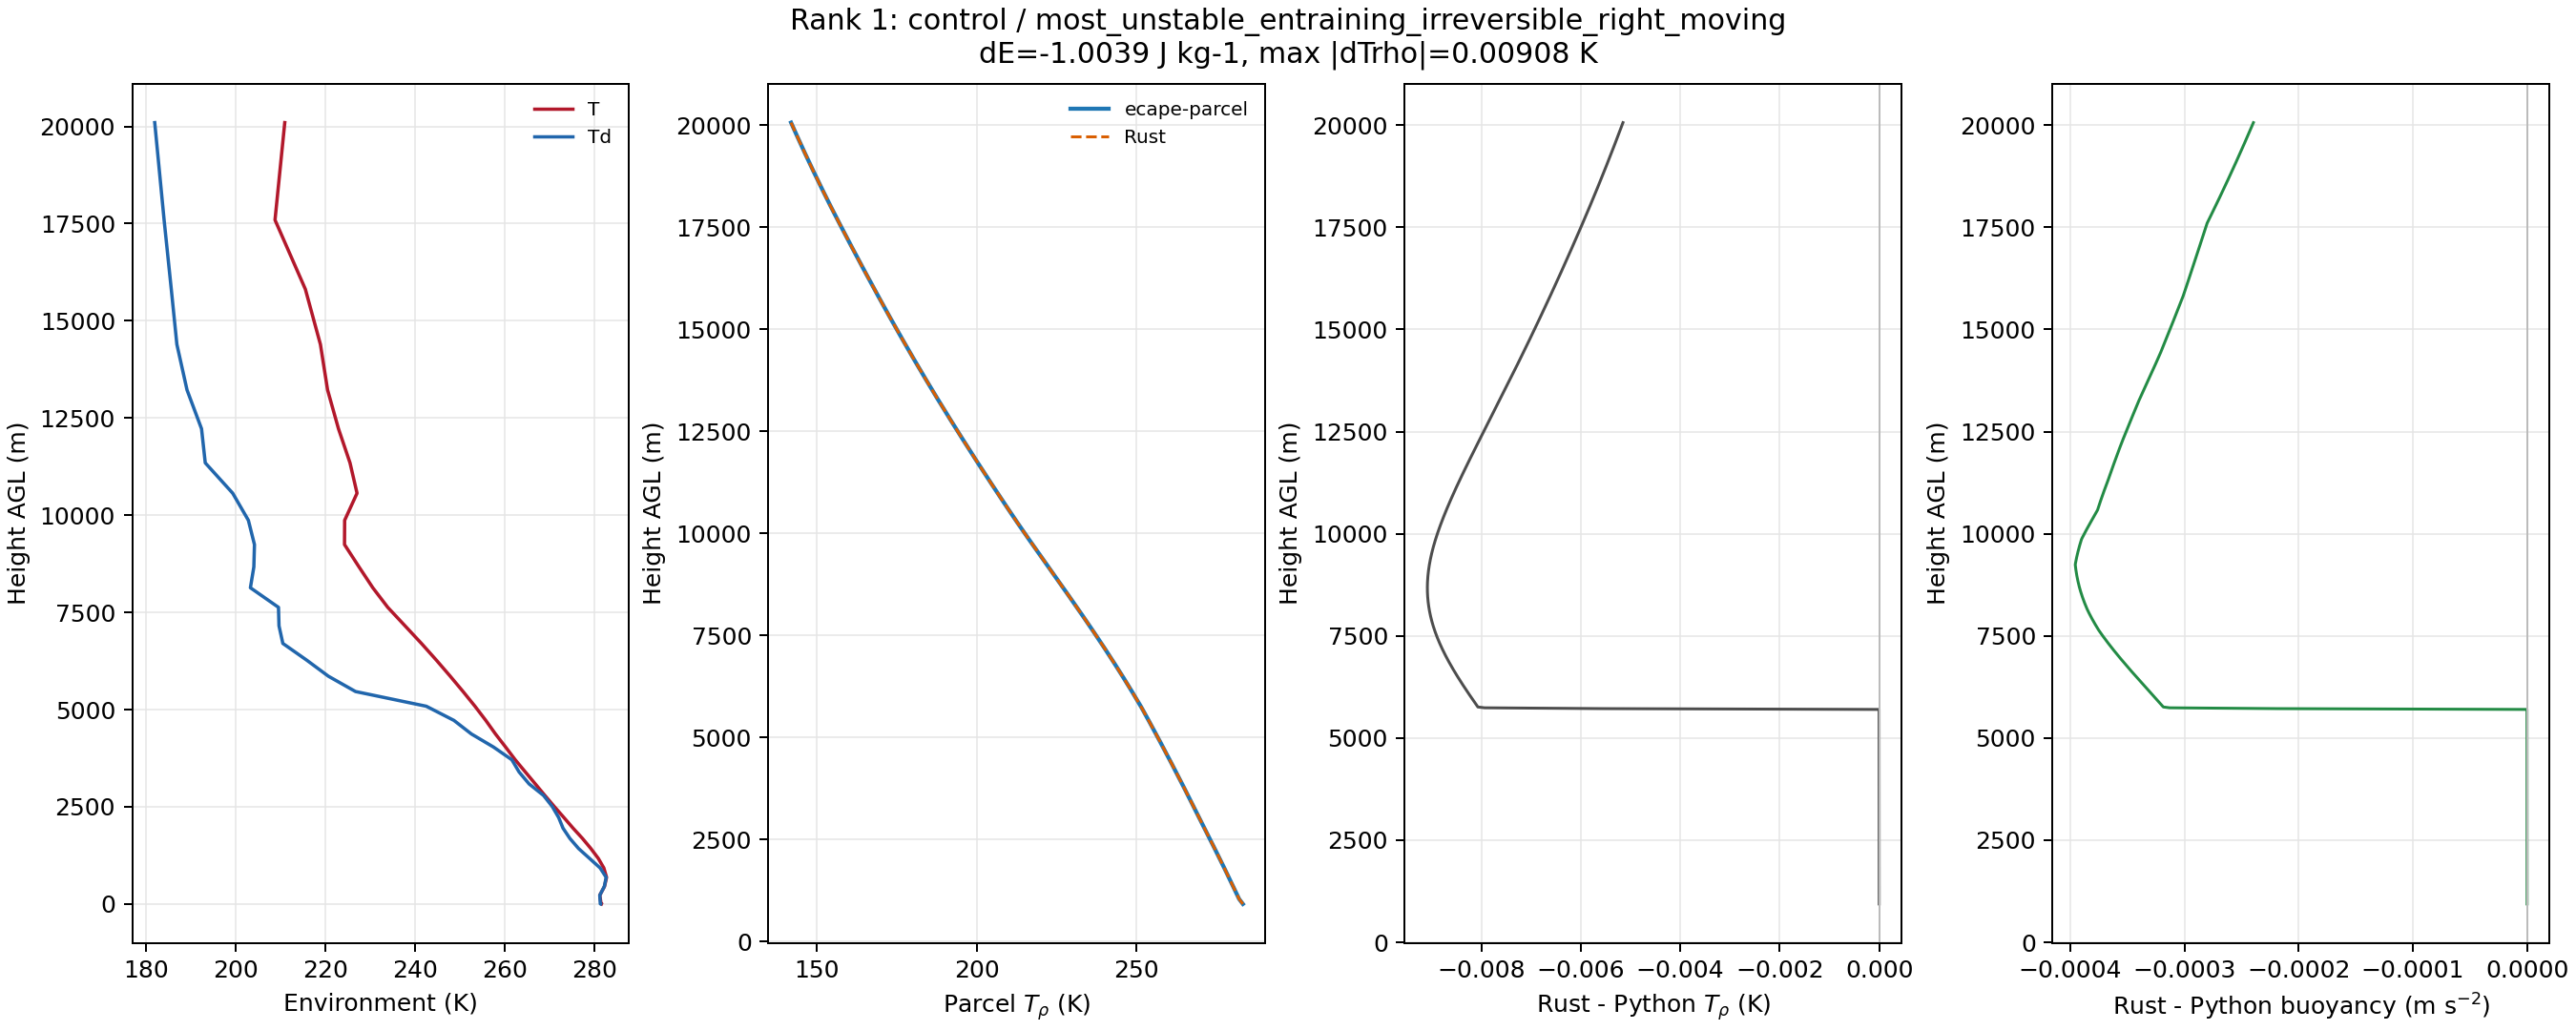
\includegraphics[width=\textwidth]{fig_worst_case_parity_control_20220305.png}
\caption{Worst event-sample parity residual from the first sweep. The largest case is a most-unstable entraining irreversible control profile from 5 March 2022. LFC and EL matched between Python and Rust, while the density-temperature residual remained within the first-stage threshold.}
\label{fig:worstcase}
\end{figure}

\begin{table}[H]
\centering
\small
\setlength{\tabcolsep}{3.5pt}
\caption{First target/control event-sample parity sweep after compatibility fixes. All 3,024 rows passed the first-stage criteria: $|\Delta E_{\mathrm{parcel}}| < \SI{2}{J\,kg^{-1}}$, maximum $|\Delta T_\rho| < \SI{0.01}{K}$, and no zero/nonzero LFC/EL or path-energy mismatch.}
\label{tab:sweep}
\begin{tabular}{lrrrrrrr}
\toprule
Sample & Profiles & Configs & Median $|\Delta E|$ & p95 $|\Delta E|$ & p99 $|\Delta E|$ & Max $|\Delta E|$ & Max $|\Delta T_\rho|$ \\
 & & & (J\,kg$^{-1}$) & (J\,kg$^{-1}$) & (J\,kg$^{-1}$) & (J\,kg$^{-1}$) & (K) \\
\midrule
Control & 200 & 2400 & 0.020 & 0.048 & 0.083 & 1.004 & 0.00908 \\
Target & 50 & 600 & 0.029 & 0.052 & 0.079 & 0.093 & 0.00045 \\
Synthetic & 1 & 12 & 0.347 & 0.399 & 0.400 & 0.401 & 0.00037 \\
HRRR test & 1 & 12 & 0.035 & 0.040 & 0.040 & 0.040 & 0.00003 \\
\bottomrule
\end{tabular}
\end{table}

\begin{table}[H]
\centering
\scriptsize
\setlength{\tabcolsep}{3pt}
\caption{The same 3,024-row sweep summarized by parcel source and ascent mode. The most stringent residual was in most-unstable entraining irreversible controls, with maximum $|\Delta E|=\SI{1.004}{J\,kg^{-1}}$ and maximum $|\Delta T_\rho|=\SI{0.00908}{K}$, still below the first-stage thresholds.}
\label{tab:bymode}
\begin{tabular}{llrrrrrr}
\toprule
Parcel & Mode & N & Median $|\Delta E|$ & p95 & p99 & Max $|\Delta E|$ & Max $|\Delta T_\rho|$ \\
 & & & (J\,kg$^{-1}$) & (J\,kg$^{-1}$) & (J\,kg$^{-1}$) & (J\,kg$^{-1}$) & (K) \\
\midrule
SB & Non-ent. irrev. & 252 & 0.018 & 0.042 & 0.053 & 0.382 & 0.00000 \\
SB & Non-ent. pseudo & 252 & 0.021 & 0.045 & 0.055 & 0.386 & 0.00000 \\
SB & Entr. irrev. & 252 & 0.018 & 0.062 & 0.097 & 0.303 & 0.00069 \\
SB & Entr. pseudo & 252 & 0.022 & 0.065 & 0.102 & 0.306 & 0.00093 \\
ML & Non-ent. irrev. & 252 & 0.018 & 0.042 & 0.052 & 0.389 & 0.00000 \\
ML & Non-ent. pseudo & 252 & 0.022 & 0.043 & 0.054 & 0.395 & 0.00000 \\
ML & Entr. irrev. & 252 & 0.017 & 0.040 & 0.066 & 0.307 & 0.00060 \\
ML & Entr. pseudo & 252 & 0.022 & 0.047 & 0.069 & 0.310 & 0.00138 \\
MU & Non-ent. irrev. & 252 & 0.026 & 0.045 & 0.055 & 0.398 & 0.00000 \\
MU & Non-ent. pseudo & 252 & 0.027 & 0.047 & 0.056 & 0.401 & 0.00000 \\
MU & Entr. irrev. & 252 & 0.025 & 0.064 & 0.137 & 1.004 & 0.00908 \\
MU & Entr. pseudo & 252 & 0.028 & 0.069 & 0.104 & 0.312 & 0.00069 \\
\bottomrule
\end{tabular}
\end{table}

A bounded second sweep added random HRRR profiles, the curated stress suite, and four storm-motion options. It produced 5,368 comparable configuration rows with zero first-stage parity failures (Table~\ref{tab:v2sweep}). One random high-terrain/dry profile triggered eight \texttt{ecape-parcel} reference exceptions in mixed-layer entraining modes, all from \texttt{dewpoint\_from\_specific\_humidity}; those reference exceptions were recorded separately and were not counted as Rust/Python parity passes or failures because Python did not return a parcel path. The other configurations from that profile still matched tightly.

\begin{table}[H]
\centering
\scriptsize
\setlength{\tabcolsep}{2.2pt}
\caption{Bounded v2 random/stress/storm-motion parity sweep. Pass rate is computed only for configurations where \texttt{ecape-parcel} returned a reference parcel path; reference exceptions are counted separately.}
\label{tab:v2sweep}
\begin{tabular}{lrrrrrrrrr}
\toprule
Sample & Profiles & Configs & Ref. exc. & Median $|\Delta E|$ & p95 & p99 & Max $|\Delta E|$ & Max $|\Delta T_\rho|$ & Pass \\
 & & & & (J\,kg$^{-1}$) & (J\,kg$^{-1}$) & (J\,kg$^{-1}$) & (J\,kg$^{-1}$) & (K) & rate \\
\midrule
Random HRRR & 100 & 4792 & 8 & 0.00085 & 0.030 & 0.038 & 0.055 & 0.00275 & 1.00 \\
Stress suite & 10 & 480 & 0 & 0.013 & 0.046 & 0.062 & 0.079 & 0.00081 & 1.00 \\
Synthetic & 1 & 48 & 0 & 0.349 & 0.401 & 0.401 & 0.401 & 0.00037 & 1.00 \\
HRRR test & 1 & 48 & 0 & 0.036 & 0.044 & 0.045 & 0.046 & 0.00008 & 1.00 \\
\bottomrule
\end{tabular}
\end{table}

\begin{table}[H]
\centering
\small
\caption{All 12 HRRR 2024-05-06 profile parity configurations after the compatibility fixes. The synthetic stress fixture also passed all 12 configurations with maximum $|\Delta E_{\mathrm{parcel}}|=\SI{0.401}{J\,kg^{-1}}$.}
\label{tab:twelvemodes}
\begin{tabular}{llrrrr}
\toprule
Parcel & Mode & $\Delta E_{\mathrm{parcel}}$ & Max $|\Delta T_\rho|$ & Python ms & Rust ms \\
 & & (J\,kg$^{-1}$) & (K) & & \\
\midrule
SB & Entraining pseudo & 0.039 & 0.00003 & 5766 & 0.482 \\
SB & Entraining irrev. & 0.035 & 0.00001 & 6086 & 0.478 \\
SB & Non-ent. pseudo & 0.035 & 0.00000 & 2778 & 0.492 \\
SB & Non-ent. irrev. & 0.034 & 0.00000 & 2905 & 0.453 \\
ML & Entraining pseudo & 0.039 & 0.00003 & 5807 & 0.484 \\
ML & Entraining irrev. & 0.036 & 0.00001 & 6121 & 0.504 \\
ML & Non-ent. pseudo & 0.035 & 0.00000 & 2772 & 0.447 \\
ML & Non-ent. irrev. & 0.034 & 0.00000 & 2843 & 0.462 \\
MU & Entraining pseudo & 0.040 & 0.00003 & 5819 & 0.653 \\
MU & Entraining irrev. & 0.039 & 0.00002 & 6019 & 0.465 \\
MU & Non-ent. pseudo & 0.036 & 0.00000 & 2776 & 0.472 \\
MU & Non-ent. irrev. & 0.035 & 0.00000 & 2837 & 0.466 \\
\bottomrule
\end{tabular}
\end{table}

\begin{figure}[H]
\centering
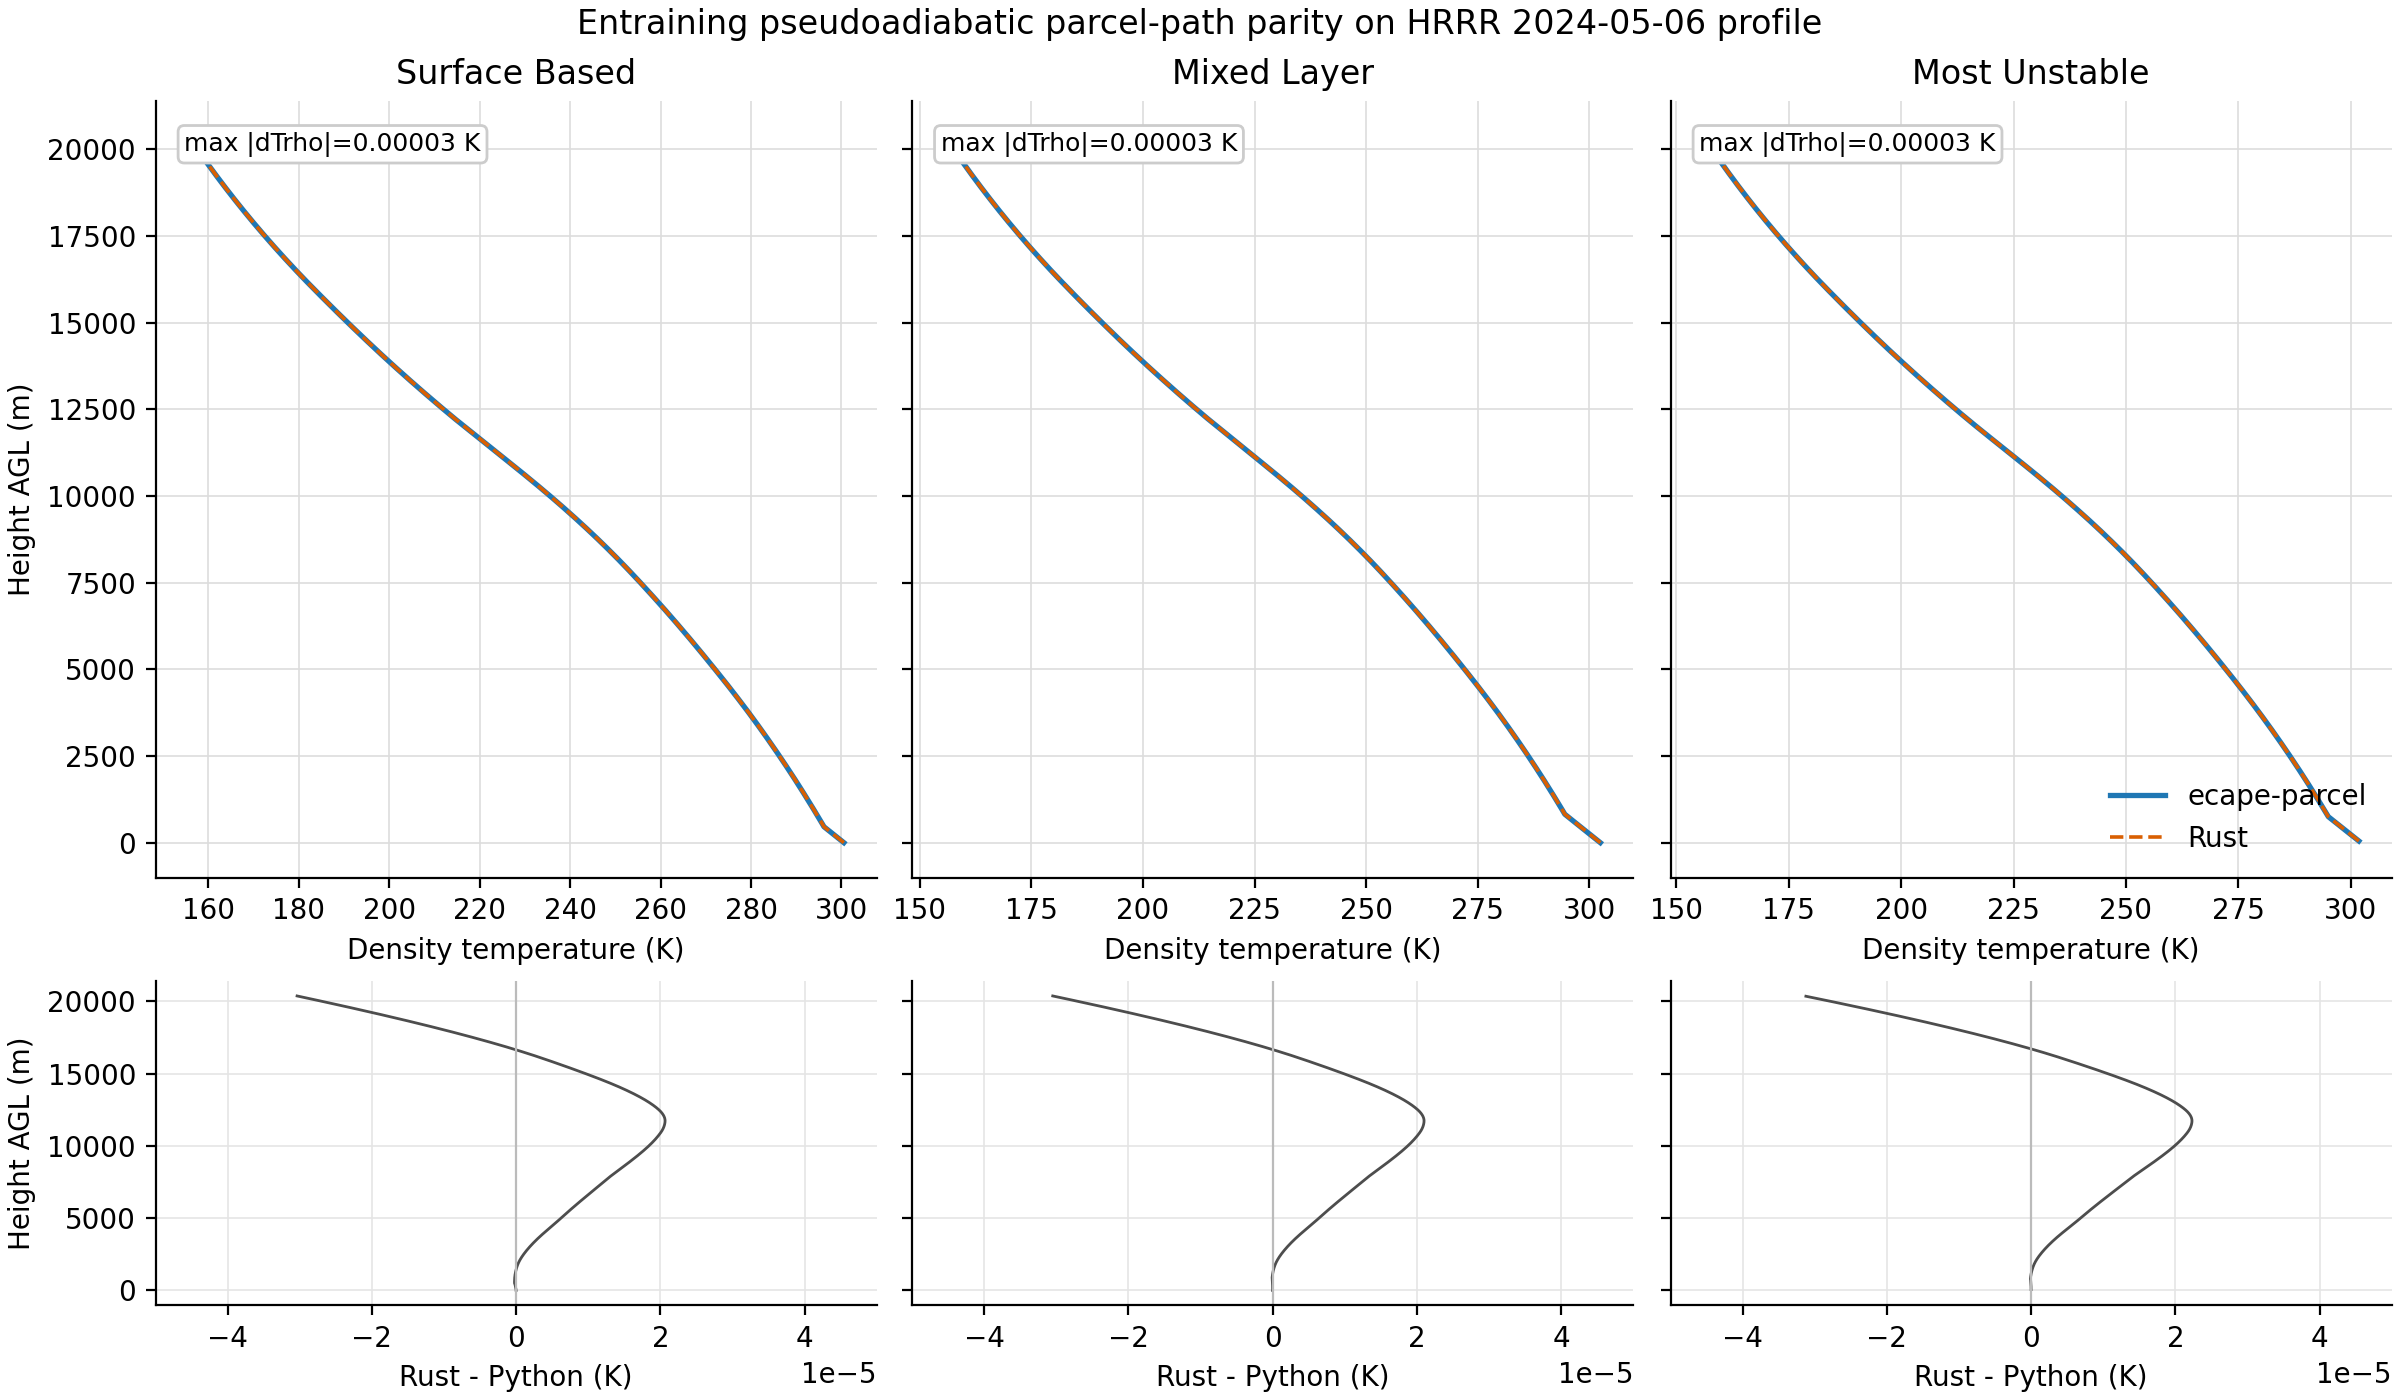
\includegraphics[width=\textwidth]{fig_ecape_parcel_parity_hrrr_20240506.png}
\caption{Direct \texttt{ecape-parcel} versus Rust density-temperature parcel paths for the HRRR 6 May 2024 warm-sector profile, using entraining pseudoadiabatic ascent.}
\label{fig:paritypaths}
\end{figure}

\section{Runtime Separation}

The benchmark must separate pure solver time from data loading, plotting, and sounding workflow overhead. In the direct parity harness, the Python \texttt{ecape-parcel} pure parcel-path call took 2.8--6.1 s per configuration on the HRRR 6 May 2024 profile, while the Rust pure call took about 0.45--0.65 ms. That benchmark implies speedups of roughly $5{,}600$--$13{,}000\times$ for that profile/configuration set.

The benchmark was run on Windows 11 using an AMD Ryzen 9 9950X3D with 16 physical cores and 32 logical processors. The software environment used Python 3.13.7, \texttt{ecape-parcel} 1.2.2, MetPy 1.7.1, NumPy 2.2.6, and Rust 1.94.0. The Python timings include the package call, Pint/MetPy unit handling, and array setup inside the call loop; the Rust timings are repeated calls to the compiled \texttt{run\_case\_raw} solver with JSON input already provided to the process. The comparison is therefore an end-to-end pure parcel-call benchmark, not a claim about total data-download or plotting speed. It is intended to represent package-level parcel-call cost in the research workflow, not an isolated language-level comparison of identical floating-point kernels.

The HRRR profile probe is a different benchmark. Its median parcel computation timer was about \SI{2}{ms}, but total profile wall time was 1.7--1.9 s because GRIB loading and profile extraction dominated. Full-grid production is different again: in the earlier full-grid pilot, four separate 272,955-cell HRRR cases each required 17.6--18.4 s per forecast hour (Table~\ref{tab:gridruntime}). These numbers should not be mixed into one headline speedup. The useful conclusion is narrower and stronger: once the HRRR data are loaded, the Rust parcel calculation is cheap enough that many parcel sources, modes, products, thresholds, and plots can be generated from the same fields.

\begin{table}[H]
\centering
\caption{Full-grid pilot runtime retained from the earlier feasibility run. Cells and wall time are per HRRR case/forecast hour; four separate cases were run. The product bundle and thread count were not isolated as a controlled benchmark, so this table is used only to document grid-scale feasibility.}
\label{tab:gridruntime}
\begin{tabular}{lrrrr}
\toprule
Workflow & Cells/case & Cases & Wall time/case & Median cells s$^{-1}$ \\
\midrule
HRRR full-grid pilot cases & 272,955 & 4 & 17.6--18.4 s & $\sim$15,400 \\
\bottomrule
\end{tabular}
\end{table}

\section{What the Speed Enables}

\subsection{Target-Control Pilot}

The 50-target/200-control pilot is not the main validation of the solver, but it shows why the solver matters. These target-control values are retained from the earlier feasibility run and are included as demonstrations of enabled analyses; they are not used as validation evidence or as final post-validation forecast-skill results. Mixed-layer tornado target points exceeded the mean of four displaced controls by \SI{383}{J\,kg^{-1}} for $E_{\mathrm{parcel}}$, \SI{373}{J\,kg^{-1}} for $E_{\mathrm{analytic}}$, and \SI{352}{J\,kg^{-1}} for the post-entrainment scalar ECAPE used in the earlier feasibility run. Mixed-layer 0--3 km ECAPE-EHI was higher by 0.96 with a 95\% bootstrap interval of 0.55--1.37.

Experimental ECAPE-EHI was defined as

\begin{equation}
\mathrm{ECAPE\text{-}EHI}_{0-3} =
\frac{E_{\mathrm{parcel}}\times \mathrm{SRH}_{0-3}}{160000}.
\end{equation}

This is a clean first composite because traditional EHI is already CAPE times SRH divided by 160,000, and the National Weather Service notes that EHI combines instability and storm-relative helicity while cautioning against magic thresholds \cite{nwsehi}. ECAPE-STP should come later because STP is a multi-term empirically tuned parameter.

\subsection{Analytic Versus Full-Path ECAPE}

After Rust/ecape-parcel parity is established on a much larger sample, the second scientific question becomes $\Delta E = E_{\mathrm{parcel}} - E_{\mathrm{analytic}}$. The current HRRR target/control sample already suggests that surface-based and mixed-layer analytic ECAPE are usually very close to full-path buoyancy but not identical. Across 250 target/control profiles, mixed-layer $E_{\mathrm{analytic}}$ and $E_{\mathrm{parcel}}$ had $r=0.99$, mean difference of \SI{37}{J\,kg^{-1}}, and mean absolute difference of \SI{95}{J\,kg^{-1}}. Most-unstable parcels had much larger outlier behavior, including cases where analytic ECAPE was zero while the parcel-path energy was nonzero. Those cases should be handled as failure-mode diagnostics before they are interpreted meteorologically.

\begin{figure}[H]
\centering
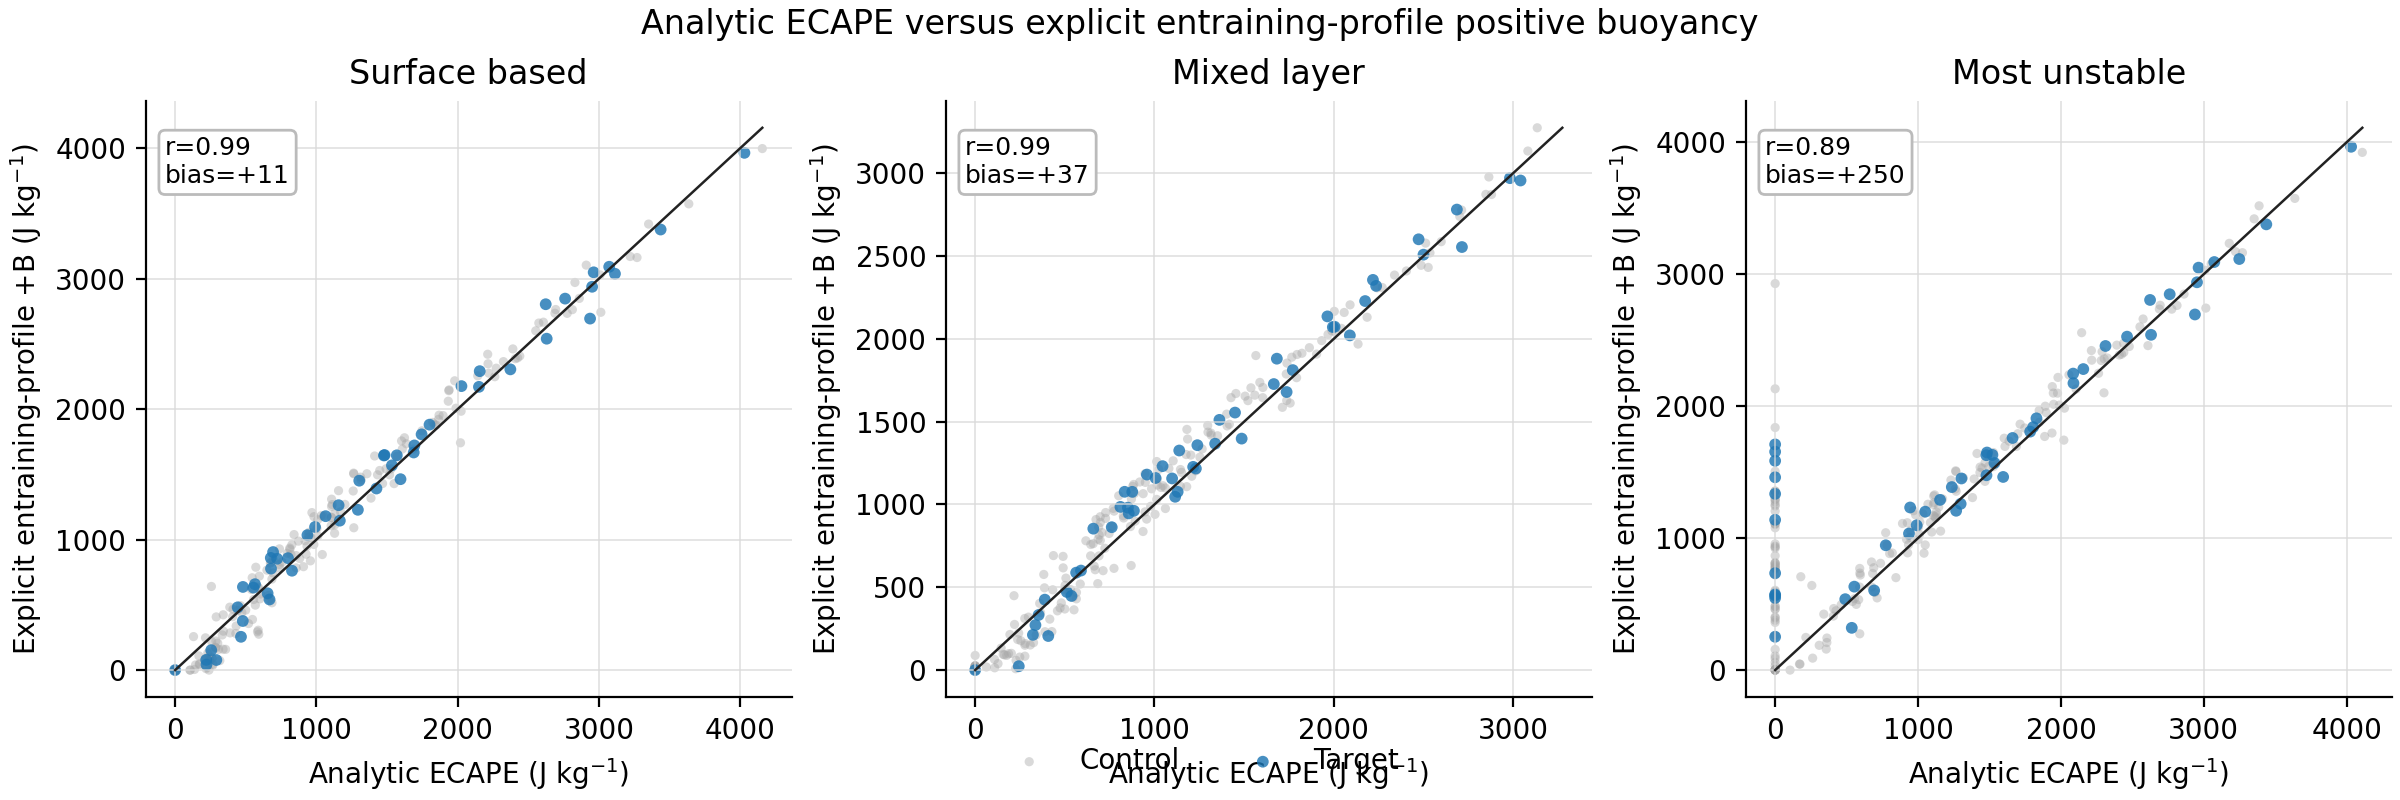
\includegraphics[width=\textwidth]{fig_analytic_vs_numerical_scatter.png}
\caption{Analytic ECAPE versus Rust parcel-path energy for the 50 target and 200 displaced-control HRRR profiles. This is now the second-stage science question, not the first validation step.}
\label{fig:analyticpath}
\end{figure}

\subsection{Full-Grid Demonstration}

The full-grid pilot changes the research object from point soundings to plumes. These grid values are also retained from the earlier feasibility run as demonstrations and are not used as validation evidence. In the 6 May 2024 case, 68.5\% of the cropped domain exceeded \SI{500}{J\,kg^{-1}} mixed-layer CAPE, 67.7\% exceeded \SI{500}{J\,kg^{-1}} mixed-layer ECAPE, and 50.1\% exceeded mixed-layer 0--3 km ECAPE-EHI of 1. In a cool-season/high-shear case on 27 February 2023, ratio fields looked large where raw CAPE was small, demonstrating why ECAPE/CAPE ratios need magnitude masks or contours.

\begin{figure}[H]
\centering
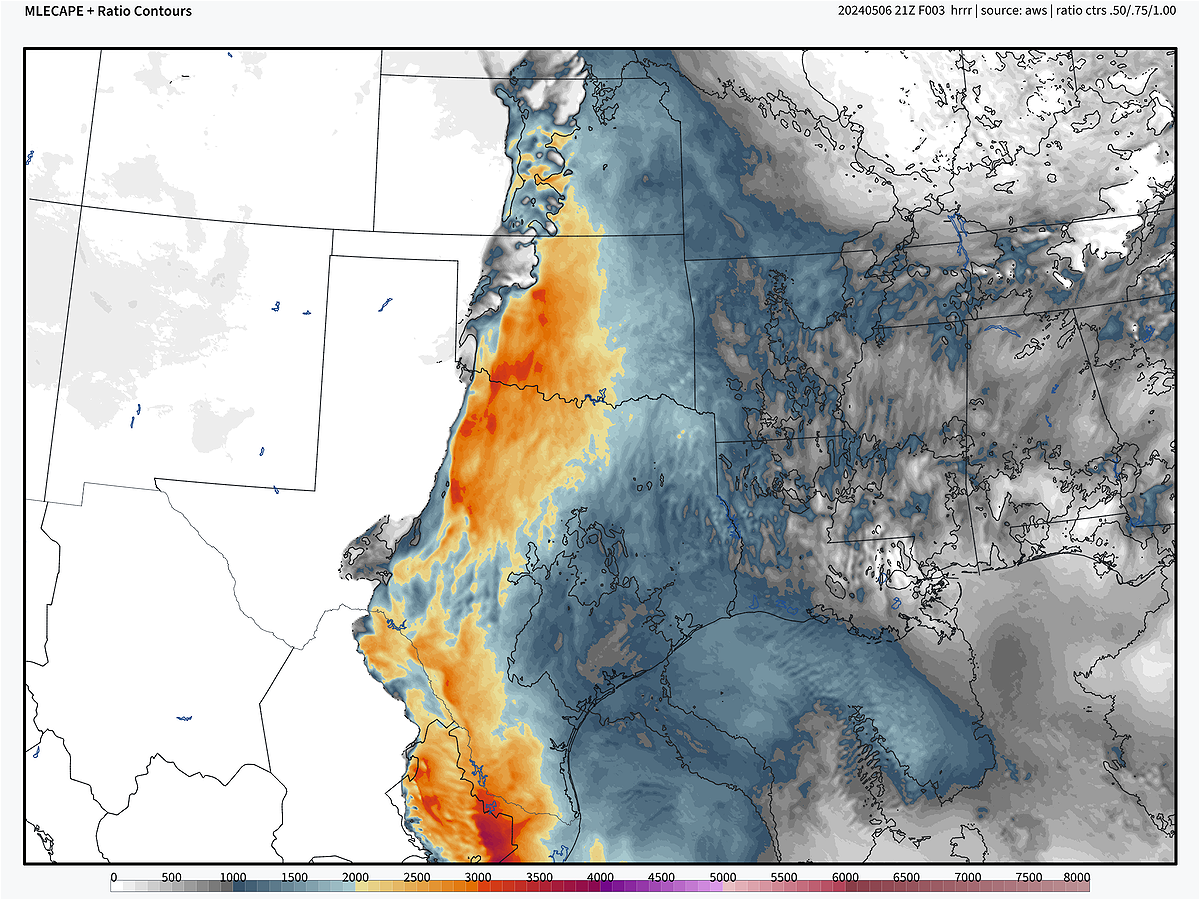
\includegraphics[width=0.90\textwidth]{fig_grid_mlecape_ratioctrs_20240506.png}
\caption{Example full-grid product from the earlier feasibility run. Ratio maps are useful only with magnitude context; the more important research direction is object-based plume verification.}
\label{fig:grid}
\end{figure}

\section{Enabled Applications and Future Validation}

High-throughput parcel-path ECAPE enables additional validation and downstream severe-weather research.

\subsection{Stage 1: ecape-parcel Compatibility and Acceleration}

The Stage 1 methods validation centers on direct \texttt{ecape-parcel} parity across surface-based, mixed-layer, most-unstable, entraining, non-entraining, pseudoadiabatic, irreversible, right-moving, left-moving, mean-wind, and user-defined storm-motion configurations. A broader validation sample should include the existing fixtures, SounderPy/ecape-parcel examples, HRRR tornado targets, displaced controls, random HRRR profiles, and hand-built stress soundings.

The current harness already found and fixed mixed-layer source construction, humidity conversion, mixed-layer dewpoint-roundtrip, most-unstable parcel-selection, zero-CAPE entraining-path, and storm-motion/VSR compatibility issues. The first target/control sweep passes across 252 profiles and 3,024 configurations. A bounded v2 sweep has also exercised random HRRR profiles, a curated stress suite, and right-moving, left-moving, mean-wind, and user-defined storm-motion modes. The remaining Stage 1 validation task is scale-up to a larger 1,000--5,000-profile random/stress sample and repetition of the full target/control archive across the full storm-motion matrix.

\subsection{Stage 2: Difference Atlas}

Once parity is established, compute $\Delta E = E_{\mathrm{parcel}} - E_{\mathrm{analytic}}$ over HRRR grids and event samples. Stratify by CAPE, CIN, LCL, EL, midlevel relative humidity, storm-relative flow, 0--1 km SRH, 0--3 km SRH, 0--6 km shear, parcel source, and storm regime. The products should include $E_{\mathrm{analytic}}$, $E_{\mathrm{parcel}}$, $\Delta E$, masked $E_{\mathrm{parcel}}/\mathrm{CAPE}$, and ECAPE-EHI.

\subsection{Stage 3: Severe-Weather Verification}

Only after Stages 1 and 2 should operational-style products be evaluated. Candidate products include ECAPE-EHI, low-level parcel-path buoyancy times SRH, masked ECAPE/CAPE ratio, recalibrated experimental ECAPE-STP, connected plume area, plume persistence, report/plume overlap, centroid displacement, and 90th/95th percentile plume intensity. Thresholds must be recalibrated; traditional EHI/STP thresholds should not be reused as if the CAPE term were unchanged.

\section{Limitations}

This is still a first-pass method pivot. The direct parity harness now covers a synthetic fixture, one HRRR 2024-05-06 warm-sector test profile, 50 tornado target profiles, 200 same-hour displaced controls, a bounded 100-profile random HRRR sample, and a curated 10-profile stress suite. It has not yet been run on a 1,000--5,000-profile random CONUS sample, and the 250 target/control profiles have not yet been repeated across the full storm-motion matrix. The harness compares against installed \texttt{ecape-parcel} 1.2.2; it does not yet call Peters's original scripts directly. The v2 sweep also exposed reference-package domain exceptions in one random profile, which should be retained as a separate reference-behavior class rather than hidden inside parity failures. The severe-weather target-control design is conservative but not a null-event verification dataset. The full-grid pilot demonstrates feasibility but not independent forecast skill. Finally, observed storm motions were not used here; recent HRRR/supercell work shows that storm-relative variables can be sensitive to observed versus estimated storm motion \cite{coffer2025gridrad}.

\section{Conclusions}

This work is best framed as high-throughput compatibility, not invention. \texttt{ecape-parcel} already made full entraining parcel-path ECAPE available for sounding-scale work. The Rust implementation makes that same class of calculation fast enough for HRRR profile batches and grid-scale products. Direct parity testing against \texttt{ecape-parcel} is now the first requirement, and the harness already improved Rust compatibility by exposing mixed-layer-origin, humidity-path, most-unstable parcel-selection, zero-CAPE, and storm-motion/VSR mismatches. After those fixes, the first target/control parity sweep passed 3,024 of 3,024 configuration rows.

The public, Peters-checked \texttt{ecape-parcel} calculation exists at sounding scale; this compatible Rust implementation makes the same class of calculation practical for HRRR-grid diagnostics. That result is scientifically useful because it enables expanded random/stress-profile parity testing, an analytic-versus-full-path ECAPE difference atlas, and eventually calibrated severe-weather verification using ECAPE-EHI and plume-object metrics.

\appendix
\section{Top Residuals From the First Event-Sample Sweep}

Table~\ref{tab:worst10} lists the ten largest absolute $E_{\mathrm{parcel}}$ residuals from the first 3,024-row sweep. The largest event-sample case is the 5 March 2022 northwest displaced-control profile shown in Fig.~\ref{fig:worstcase}; the remaining largest residuals are from the synthetic parity-column fixture and have matching paths to numerical precision, with the residual coming from integral convention differences rather than a density-temperature path offset. Here ``integral convention'' is used only when the parcel density-temperature and buoyancy paths agree to numerical precision, LFC/EL and empty-path flags match, and the remaining scalar difference is confined to the numerical treatment of the path integral: positive-buoyancy clipping, LFC/EL endpoint inclusion, and bracketing/trapezoid treatment near the first and last positive-buoyancy levels.

\begin{table}[H]
\centering
\scriptsize
\setlength{\tabcolsep}{2.5pt}
\caption{Top ten absolute $E_{\mathrm{parcel}}$ residuals from the first event-sample parity sweep.}
\label{tab:worst10}
\begin{tabular}{rllrrll}
\toprule
Rank & Case & Mode & $\Delta E$ & $\max|\Delta T_\rho|$ & LFC/EL & Reason \\
 & & & (J\,kg$^{-1}$) & (K) & match & \\
\midrule
1 & control NW 20220305 & MU EI right & -1.004 & 0.00908 & yes & upper-path residual \\
2 & synthetic column & MU NP user & +0.401 & 0.00000 & yes & integral convention \\
3 & synthetic column & MU NI user & +0.398 & 0.00000 & yes & integral convention \\
4 & synthetic column & ML NP user & +0.395 & 0.00000 & yes & integral convention \\
5 & synthetic column & ML NI user & +0.389 & 0.00000 & yes & integral convention \\
6 & synthetic column & SB NP user & +0.386 & 0.00000 & yes & integral convention \\
7 & synthetic column & SB NI user & +0.382 & 0.00000 & yes & integral convention \\
8 & synthetic column & MU EP user & +0.312 & 0.00035 & yes & integral convention \\
9 & synthetic column & MU EI user & +0.311 & 0.00037 & yes & integral convention \\
10 & synthetic column & ML EP user & +0.310 & 0.00035 & yes & integral convention \\
\bottomrule
\end{tabular}
\end{table}

Mode abbreviations in Table~\ref{tab:worst10} use E/N for entraining or non-entraining and P/I for pseudoadiabatic or irreversible ascent.

\begin{thebibliography}{9}

\bibitem{peters2023ecape}
Peters, J. M., D. R. Chavas, C.-Y. Su, H. Morrison, and B. E. Coffer, 2023:
An analytic formula for entraining CAPE in midlatitude storm environments.
\textit{Journal of the Atmospheric Sciences}, \textbf{80}, 2165--2186.
\url{https://doi.org/10.1175/JAS-D-23-0003.1}

\bibitem{ecapeparcel}
Urquhart, A. R. H., cited 2026:
\texttt{ecape-parcel} 1.2.2: A simple Python package that computes entrainment CAPE parcels.
\url{https://pypi.org/project/ecape-parcel/}

\bibitem{sounderpyparcels}
Gillett, K., cited 2026:
SounderPy plotting data documentation: parcel logic and ECAPE parcel plotting.
\url{https://kylejgillett.github.io/sounderpy/plottingdata.html}

\bibitem{hrrrweb}
NOAA Global Systems Laboratory, cited 2026:
The High-Resolution Rapid Refresh (HRRR).
\url{https://rapidrefresh.noaa.gov/hrrr/}

\bibitem{nwsehi}
National Weather Service, cited 2026:
Weather Spotter's Field Guide glossary: Energy Helicity Index.
\url{https://www.weather.gov/spotterguide/glossary_e}

\bibitem{coffer2025gridrad}
Coffer, B., M. Parker, M. Coniglio, and C. Homeyer, 2025:
Supercell environments using GridRad-Severe and the HRRR: Addressing discrepancies between prior tornado datasets.
\textit{arXiv:2503.15466}.
\url{https://arxiv.org/abs/2503.15466}

\end{thebibliography}

\end{document}
